\documentclass[10pt,twocolumn,letterpaper]{article}

\usepackage{cvpr}
\usepackage{times}
\usepackage{epsfig}
\usepackage{graphicx}
\usepackage{amsmath}
\usepackage{amssymb}
\usepackage{float}
\usepackage{listings}
\usepackage{color} %red, green, blue, yellow, cyan, magenta, black, white
\definecolor{mygreen}{RGB}{28,172,0} % color values Red, Green, Blue
\definecolor{mylilas}{RGB}{170,55,241}
\usepackage{blindtext}

% Include other packages here, before hyperref.

% If you comment hyperref and then uncomment it, you should delete
% egpaper.aux before re-running latex.  (Or just hit 'q' on the first latex
% run, let it finish, and you should be clear).
\usepackage[breaklinks=true,bookmarks=false]{hyperref}

\cvprfinalcopy % *** Uncomment this line for the final submission

\def\cvprPaperID{****} % *** Enter the CVPR Paper ID here
\def\httilde{\mbox{\tt\raisebox{-.5ex}{\symbol{126}}}}

% Pages are numbered in submission mode, and unnumbered in camera-ready
%\ifcvprfinal\pagestyle{empty}\fi
\setcounter{page}{1}
\begin{document}

%%%%%%%%% TITLE
\title{Machine Learining for Computer Vision Coursework 1\\
	Face Recognition by PCA
	}

\author{David Angelov\\
MEng Electrical and Electronic Engineering \\
Imperial College London\\
{\tt\small david.angelov12@imperial.ac.uk}
% For a paper whose authors are all at the same institution,
% omit the following lines up until the closing ``}''.
% Additional authors and addresses can be added with ``\and'',
% just like the second author.
% To save space, use either the email address or home page, not both
\and
Huaqi Qiu\\
MSc Communication and Signal Processing\\
Imperial College London\\
{\tt\small h.qiu15@imperial.ac.uk}
}

\maketitle
%\thispagestyle{empty}

%%%%%%%%% BODY TEXT
\section{Question 1}
In this coursework, we were given 10 normalized and vectorized face images for each of the 52 different people (referred to as 'class' in this report). Firstly, the given data set was separated into training data and testing data. In this coursework, 80\% of data was used for the purpose of training and 20\% of data were used for training. The partition was done by randomly selecting 8 out of 10 images for training. Naturally, the remaining 2 images in each class were used for testing. This partition method ensured the randomness of the data sets and full coverage of classes.\\
\\
Next, we applied PCA to the training data by projecting the faces to so called face space, which is spanned by M eigenfaces. To acquire the eigenfaces, we started with computing the mean face $\boldsymbol{\bar{x}}$ from the $n$ training images $x_n$ by
\begin{equation}
 \boldsymbol{\bar{x}} = \frac{1}{N} \sum_{n=1}^N \boldsymbol{x_n}
 \label{eq:mean_face}
\end{equation}

and the resulting mean face image is shown in Figure~\ref{fig:q1_meanface}. 


\begin{figure}[H]
	\begin{center}
		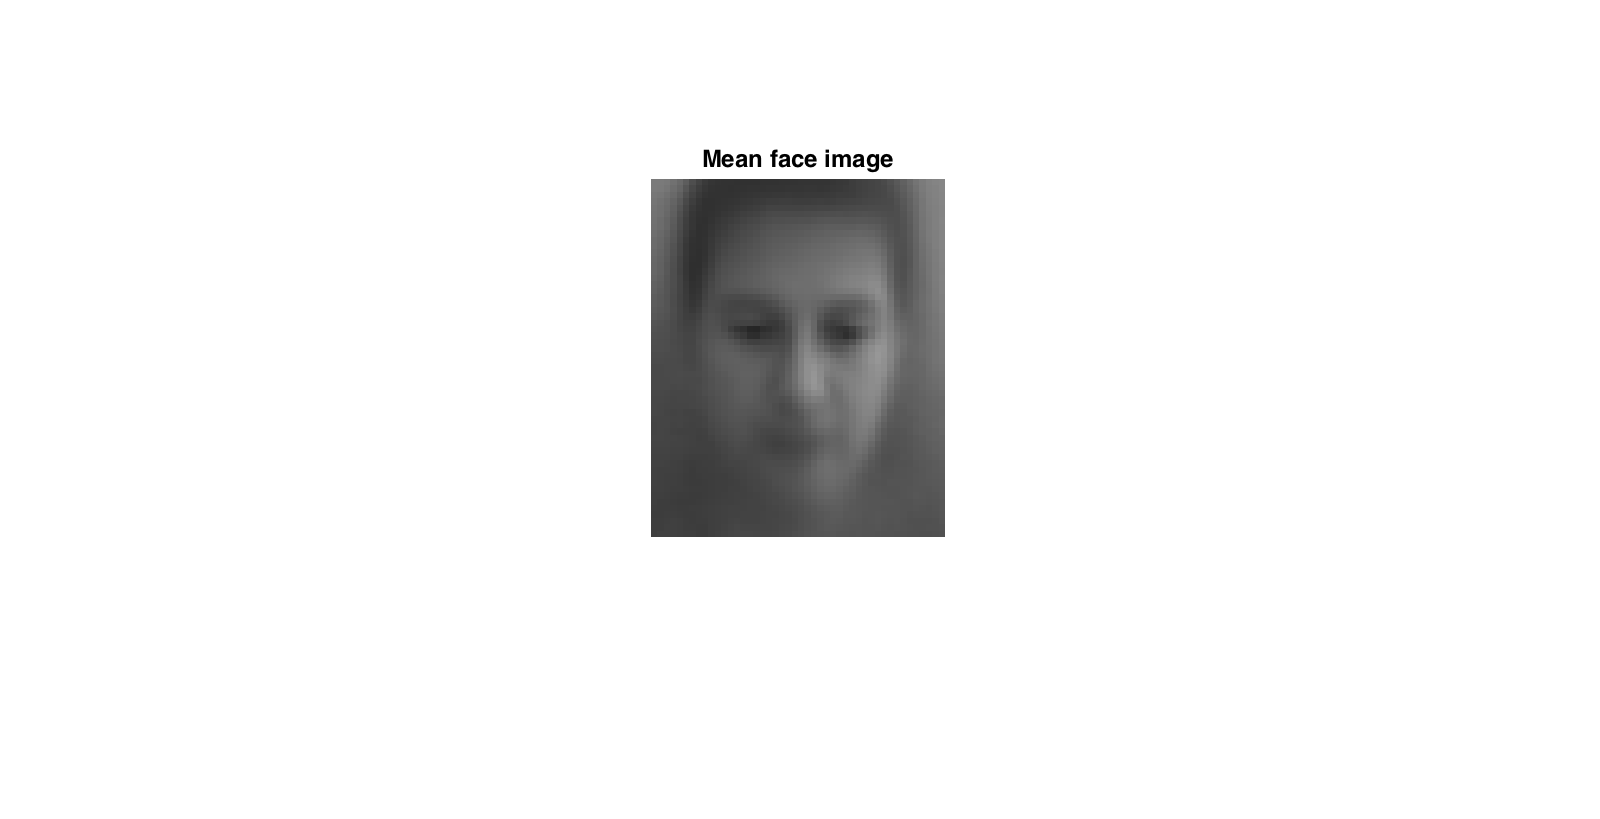
\includegraphics[width=0.8\linewidth]{q1_meanface}
		\caption{Mean face}
	\end{center}
	\label{fig:q1_meanface}
\end{figure}


Then, the all training faces were normalized by subtracting the mean face

\begin{equation}
\boldsymbol{\phi}_n = \boldsymbol{x_n} - \boldsymbol{\bar{x}}
\label{eq:q1_phi}
\end{equation}

and the matrix $\boldsymbol{A}$ can be acquired by

\begin{equation}
\boldsymbol{A} = [\phi_1, \phi_2, ..., \phi_N]
\label{eq:q1_A}
\end{equation}

Then the covariance matrix was calculated by

\begin{equation}
	\boldsymbol{S} = \frac{1}{N} A A^T
	\label{eq:q1_S}
\end{equation}

The eigenvectors $\boldsymbol{u_i}$ were calculated from the covariance matrix $S$ by $\boldsymbol{S u_i} = \lambda_i \boldsymbol{u_i}$. The dimension of the training data vector $x_n$ is $D = 2576$, denoted by $x_n \in R^D$ (for the data provided for this coursework). To reduce the dimension and maximising the variance of projected data, we selected M of the eigenvectors corresponding to the M largest eigenvalues $\lambda_i$ as eigenfaces. We found that among all the $\lambda_i$ ($i = 1,2, ..., D$), 415 out D eigenvalues were considered large (or non-zero), with order of magnitude ranging from 1 to 5. The remaining $D - 415 = 2161$ of the eigenvalues were considered as zeros with order of magnitude ranging from -10 to -13. In this coursework, we selected the largest $M = 50$ eigenfaces as the basis vectors for the face space. In Figure~\ref{fig:eigFaces}, we visualised 16 out of these 50 eigenfaces. The eigenfaces were visualised by reshaping the $x_n$ vector to a $54 \times 46$ matrix.

\begin{figure}
	\begin{center}
		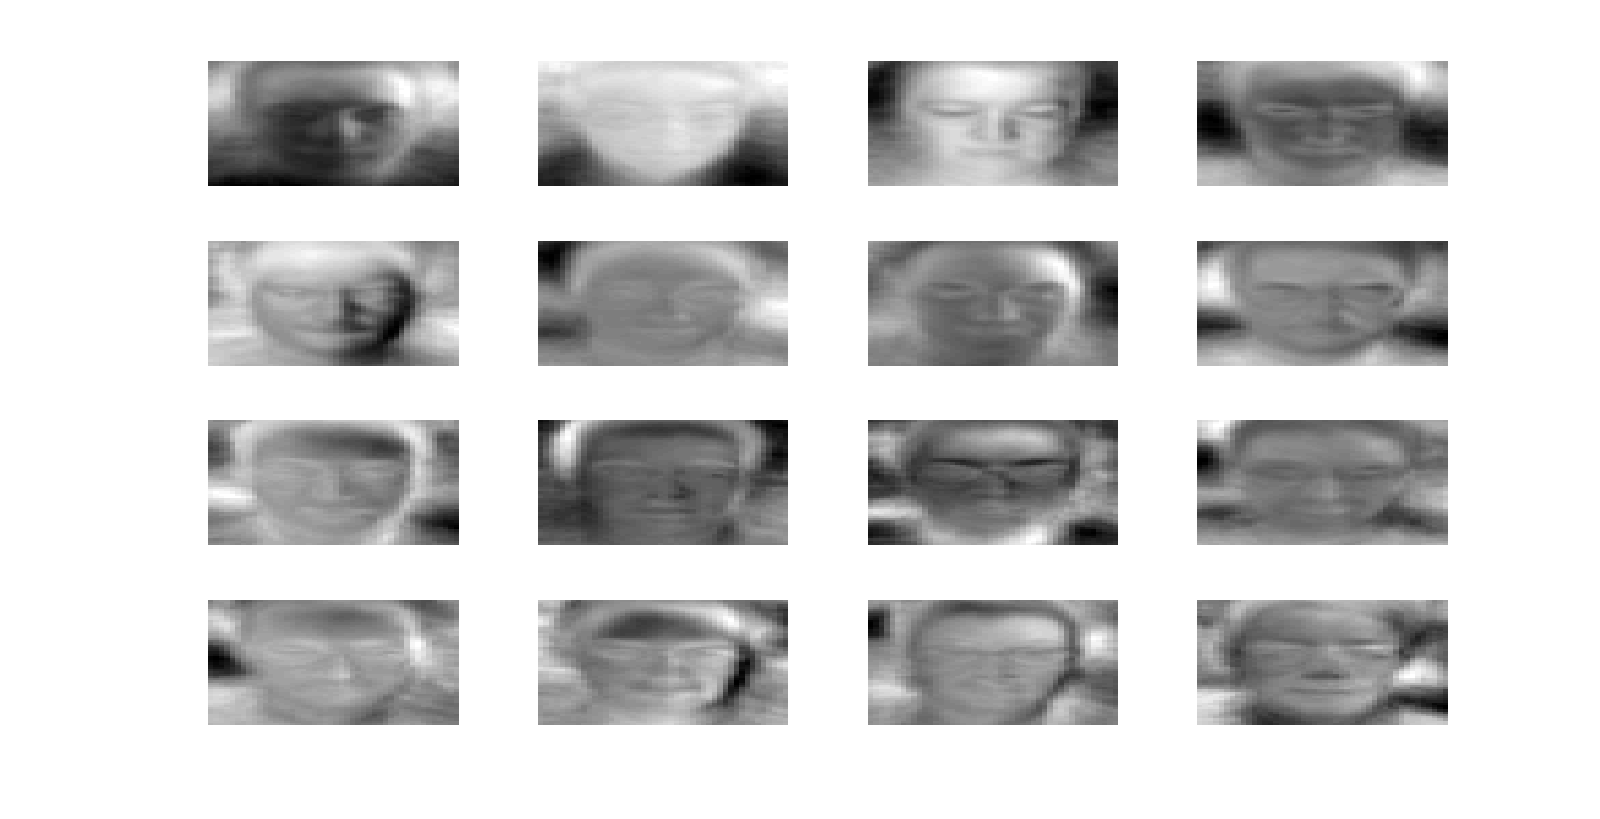
\includegraphics[width=0.8\linewidth]{q1_eigenfaces}
		\caption{The first 16 eigenfaces visualised}
		\label{fig:eigFaces}
	\end{center}
\end{figure}

To apply the PCA method, we projected every normalised training face $\phi_n$ to the M-dimensional subspace. Namely,
\begin{equation}
\omega_n = [a_{n1}, a_{n2}, ..., a_{nM}]
\label{eq:project}
\end{equation}

where the projection of $n$th image on the $i$th eigenface is denoted by

\begin{equation}
a_{ni} = \phi_n^T \boldsymbol{u_i}, ~  i = 1,...,M
\label{eq:project_a}
\end{equation}


Thus, the training faces were represented by its projections $\omega_n$. \\


\section{Question 2}
In this question, we discuss two different methods of calculating covariance matrix $S$ in the scope of PCA. It can be noticed from Eq.\ref{eq:q1_S} that the dimension of the covariance matrix is $D\times D$, which equals to the number of pixels in an image and is typically large. Under the consideration of computational efficiency, we implemented another proposed method, in which the covariance matrix is calculated by

\begin{equation}
S = \frac{1}{N} A^T A
\label{eq:S_q2}
\end{equation}

Since $A \in R^{D \times N}$, the covariance matrix now has dimension of $N \times N$, where $N$ equals to the number of images and is typically much smaller than $D$. As computing eigenvectors of large matrices is computational expensive, this method is preferred if proved equally effective for PCA. The resulting none-zero eigenvalues from Eq.\ref{eq:S_q2} had the same value of that using Eq.\ref{eq:q1_S}. The number of non-zero eigenvalues in this case is also 415. Note that the eigenvectors using this method were converted to the D-dimensional eigenvectors by 

\begin{equation}
	\boldsymbol{u_i} = A \boldsymbol{v_i}
\end{equation}

where $v_i$ denotes the eigenvectors calculated using the covariance matrix in Eq.\ref{eq:S_q2}. Figure~\ref{fig:q2_eigFaces} shows the visualised 16 eigenfaces. Comparing to the eigenfaces produced by the previous method (Figure~\ref{fig:eigFaces}), we notice that the face contour of the eigenfaces are the same. The difference in grey scale value could be caused by the randomisation of the data set and automatic normalisation by the image display function \texttt{imagesc} in MATLAB.\\

In conclusion, the methods for the computation of covariance matrix in Q1 and Q2 were proven equally effective for PCA, while the latter method is less computational expensive. Hence we used $S = (1/N) A^T A$ to compute the covariance matrix for image recognition in later sections of this coursework.


\begin{figure}
	\begin{center}
		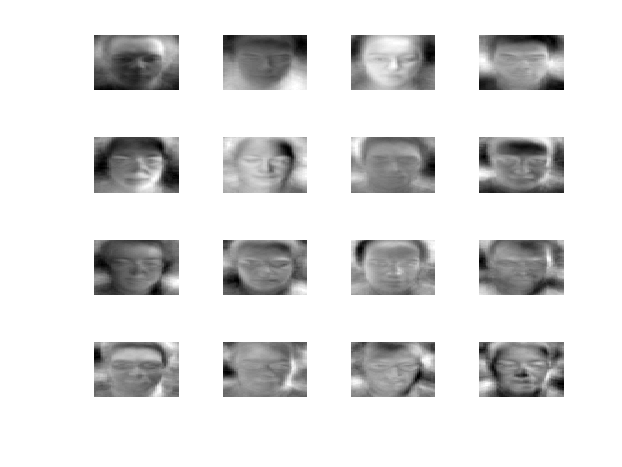
\includegraphics[width=1\linewidth]{q2_eigenfaces}
		\caption{The first 16 eigenfaces visualised for question 2}
		\label{fig:q2_eigFaces}
	\end{center}
\end{figure}

%\begin{figure*}
%\begin{center}
%\fbox{\rule{0pt}{2in} \rule{.9\linewidth}{0pt}}
%\end{center}
 %  \caption{Example of a short caption, which should be centered.}
%\label{fig:short}
%\end{figure*}

%------------------------------------------------------------------------
\section{Question 3}
The face images can be reconstructed from their projection on the M-dimensional subspace $\omega_n$ by

\begin{equation}
	\boldsymbol{\widetilde{x_n}} = \boldsymbol{\bar{x}} + \sum_{i=1}^M a_{ni} \boldsymbol{u_i}
\end{equation}

where $\boldsymbol{\widetilde{x_n}}$ is the reconstructed face image. The reconstruction error, denoted as $J$ can be evaluated by

\begin{equation}
 J = \frac{1}{N} \sum_{n=1}^N || \boldsymbol{x_n} - \boldsymbol{\widetilde{x_n}}||^2
 \label{eq:J}
\end{equation}

where N is the total number of images. The formulation of PCA that we applied in this coursework maximises the variance of the projection of training data by spanning the face space using M eigenvectors $\{ \boldsymbol{u_i} \}$ of $S$ corresponding to the largest M eigenvalues $\{ \lambda_i \}$ where ($i = 1,2,...,M$). This formulation equivalently minimises the reconstruction error $J$ so it theoretically becomes

\begin{equation}
J_{theo} = \sum_{i=M+1}^{D^*} \lambda_i
\label{eq:J_theo}
\end{equation}

The $D^*$ in Eq.\ref{eq:J_theo} is the total number of eigenvectors of $S$. For the method we selected in Question 2, $D^* = 416$, which equals to the total number of training images. We evaluated and compared the experimental $J$ calculated by Eq. \ref{eq:J} and theoretical $J_{theo}$ calculated by Eq.\ref{eq:J_theo} while varying the number of M. Figure~\ref{fig:q3_J} presents $J$ and $J_{theo}$ as M varying from 40 to 100.\\
	
	\begin{figure}
		\begin{center}
			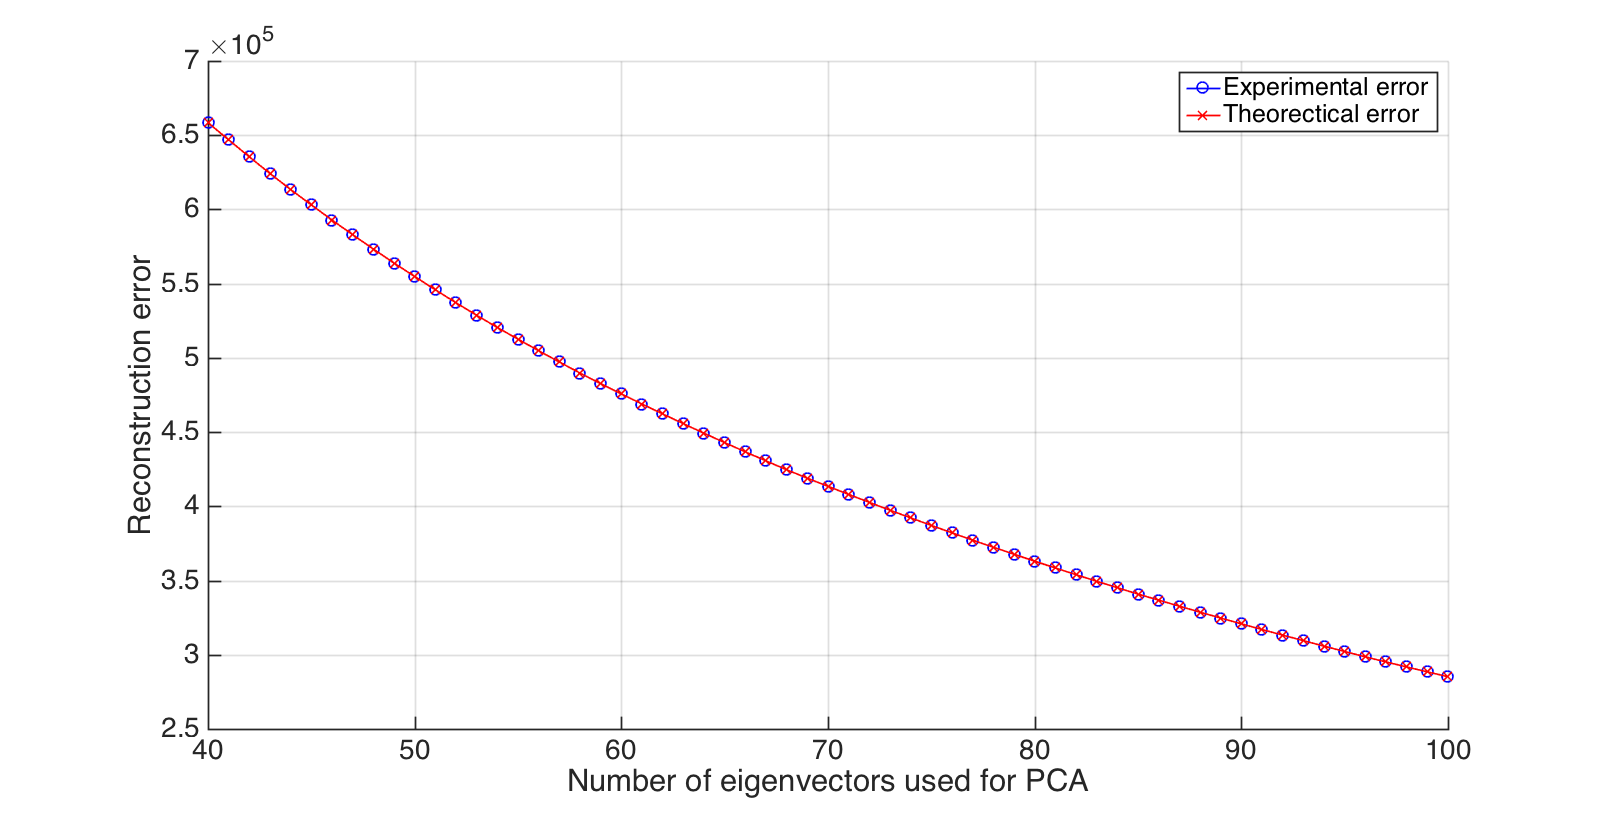
\includegraphics[width=1\linewidth]{q3_J}
			\caption{Reconstruction error, experimental vs theoretical}
			\label{fig:q3_J}
		\end{center}
	\end{figure}

It can be noticed that 1) the theoretical and experimental reconstruction errors are identical for all value of M; 2) the reconstruction error reduces when the number of M increases, but the gradient of the decreasing error curve reduces. This indicates that the positive effect of using more number of eigenfaces on reducing $J$ decreases as M increases. 

Figure~\ref{fig:q3_rec_train} shows the original training faces and the corresponding reconstructed images. Similarly, Figure~\ref{fig:q3_rec_test} shows the original testing faces and corresponding reconstructed images. As we can observe, the face images were well-reconstructed for both training and testing faces.
	
	\begin{figure}
		\begin{center}
			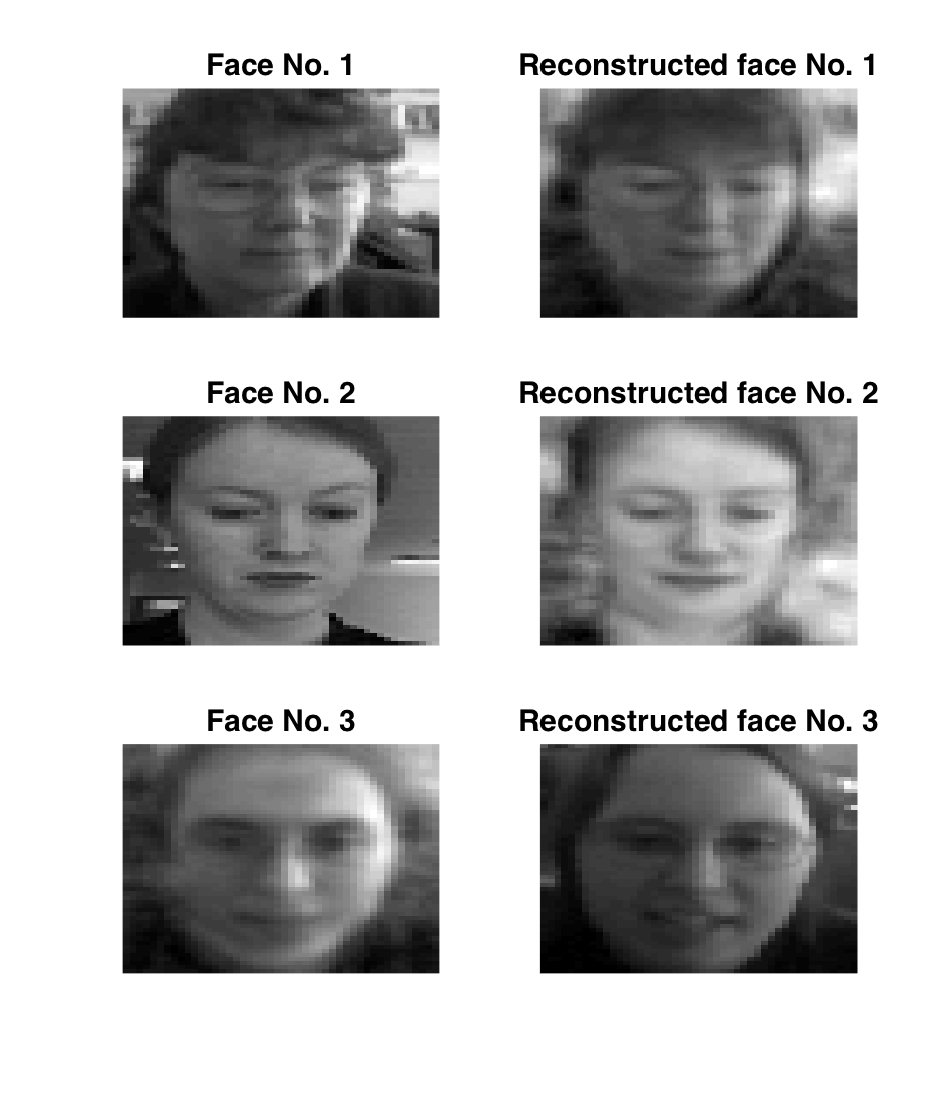
\includegraphics[width=1\linewidth]{q3_rec_train}
			\caption{Visualise reconstructed training images}
			\label{fig:q3_rec_train}
		\end{center}
	\end{figure}
	
	
	\begin{figure}
		\begin{center}
			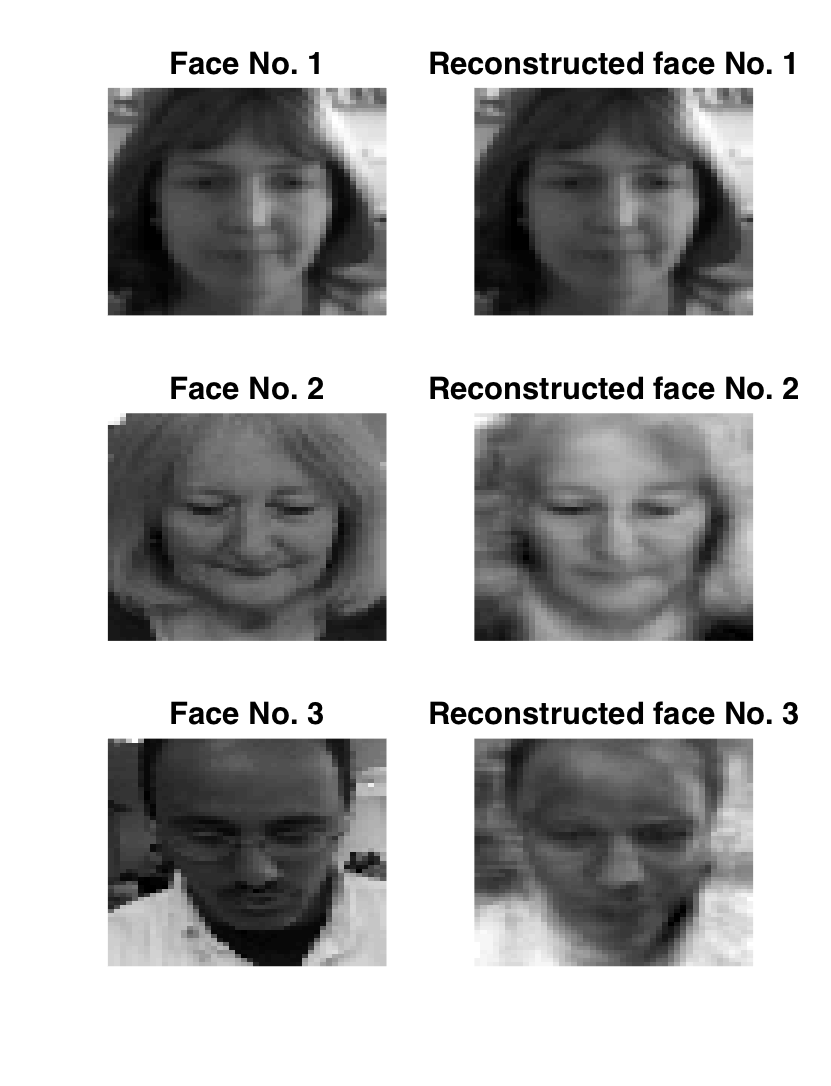
\includegraphics[width=1\linewidth]{q3_rec_test}
			\caption{Visualise reconstructed testing images}
			\label{fig:q3_rec_test}
		\end{center}
	\end{figure}

\section{Question 4}
At the training stage, the training images were projected on the M-dimensional face space. The $n^{th}$ image in the training set was represented  as $\omega_n$. At testing stage, each testing image was normalised by Eq.\ref{eq:q1_phi} and then projected on the eigenspace by Eq.\ref{eq:project_a} and represented as

$$ \omega = [a_1, a_2, ..., a_M]^T$$

This process transformed the testing images to represented data points that can be classified to a specific image in training set, thus effectively, recognised. In this coursework, the classification was achieved by Nearest Neighbour method and Alternative method. We shall now discuss and compare the two methods.

\subsection{Nearest Neighbour classification}
In the Nearest Neighbour (NN) classification, the testing image is assigned to the class which has the minimum error $e$, which is calculated with respect to all training images as

\begin{equation}
	e = || \omega - \omega_n||, ~ n = 1, ..., N
\end{equation}
where recall N is the number of training images. 







\subsection{Alternative method for classification}


{\small
\bibliographystyle{ieee}
\bibliography{egbib}
}

\onecolumn
\appendix
\section{Appendix 1 Matlab Code}
\subsection{Init.m}
\lstinputlisting{init.m}

\section{matlab code part 2}
\lstinputlisting{init.m}



\end{document}
